\documentclass[conference]{IEEEtran}
\IEEEoverridecommandlockouts

% Packages
\usepackage{cite}
\usepackage{amsmath,amssymb,amsfonts}
\usepackage{algorithmic}
\usepackage{graphicx}
\usepackage{textcomp}
\usepackage{xcolor}
\usepackage{url}
\usepackage{booktabs}
\usepackage{listings}
\usepackage{subcaption}

% Configure listings for code
\lstset{
    basicstyle=\footnotesize\ttfamily,
    breaklines=true,
    frame=single,
    showstringspaces=false,
    commentstyle=\color{gray},
    keywordstyle=\color{blue},
    stringstyle=\color{red}
}

\def\BibTeX{{\rm B\kern-.05em{\sc i\kern-.025em b}\kern-.08em
    T\kern-.1667em\lower.7ex\hbox{E}\kern-.125emX}}

\begin{document}

\title{SDLP: A Lightweight Protocol for Authenticated Deep Links with Decentralized Identity}

\author{
\IEEEauthorblockN{Prem Pillai}
\IEEEauthorblockA{\textit{AI Engineer} \\
Melbourne, Australia \\
prem.pillai@gmail.com}
}

\maketitle

\begin{abstract}
Deep links enable seamless inter-application communication by encoding data directly within URLs, but they lack inherent security mechanisms to verify sender authenticity or payload integrity. This paper introduces the Secure Deep Link Protocol (SDLP), a lightweight protocol that provides cryptographic authentication and integrity verification for data transmitted via deep links. SDLP leverages JSON Web Signatures (JWS) with Ed25519 cryptography and Decentralized Identifiers (DIDs) to create verifiable links without requiring centralized certificate authorities. Our protocol achieves 72\% payload efficiency within typical URL length constraints and supports flexible compression algorithms. Performance evaluation shows sub-millisecond link creation (0.09-0.11ms average) and verification times (0.32-0.38ms average) with throughput exceeding 9,000 operations per second. SDLP addresses critical security gaps in deep link communication while maintaining compatibility with existing URL schemes and mobile application ecosystems.
\end{abstract}

\begin{IEEEkeywords}
deep links, authentication, decentralized identity, mobile security, cryptographic protocols, JSON Web Signature
\end{IEEEkeywords}

\section{Introduction}

Deep links serve as a fundamental mechanism for inter-application communication in modern computing environments, particularly in mobile ecosystems where they enable applications to invoke specific functionalities with contextual data~\cite{android-app-links, ios-universal-links}. However, standard deep links present significant security vulnerabilities: they lack mechanisms to verify the sender's authenticity or ensure payload integrity, making them susceptible to spoofing, injection attacks, and data manipulation.

Consider these attack scenarios: A malicious actor could craft deep links containing harmful prompts for AI applications, manipulate configuration parameters in development tools, or inject unauthorized commands into automation systems. These vulnerabilities become particularly concerning as deep links increasingly carry sensitive data such as API tokens, user preferences, or executable configurations.

Existing solutions like JWT tokens embedded in URLs suffer from substantial overhead (approximately 78\% size penalty due to double Base64URL encoding), while traditional PKI-based approaches require centralized certificate authorities that may not be available or appropriate for peer-to-peer scenarios.

This paper presents the Secure Deep Link Protocol (SDLP), which addresses these limitations through the following contributions:

\begin{enumerate}
    \item A lightweight protocol design that separates cryptographic metadata from payload data to minimize URL overhead
    \item Integration with Decentralized Identifiers (DIDs) for sender authentication without centralized authorities
    \item Comprehensive performance evaluation demonstrating sub-millisecond operation latencies
    \item Open-source reference implementation with production-ready benchmarking suite
\end{enumerate}

\section{Related Work}

\subsection{Deep Link Security}

Traditional deep linking mechanisms in mobile platforms rely on custom URL schemes (iOS) or intent filters (Android) without built-in authentication~\cite{android-intents, ios-url-schemes}. While Universal Links~\cite{ios-universal-links} and App Links~\cite{android-app-links} provide domain-based verification, they require web server control and don't address payload integrity.

Recent work has explored authenticated deep links for specific use cases. OAuth 2.0 for native applications~\cite{rfc8252} uses deep links for authorization flows but focuses on token exchange rather than general payload transmission. Mobile app security frameworks~\cite{mobile-app-security} identify deep link vulnerabilities but don't provide comprehensive solutions.

\subsection{JSON Web Signatures and Tokens}

JSON Web Signatures (JWS)~\cite{rfc7515} and JSON Web Tokens (JWT)~\cite{rfc7519} provide established patterns for cryptographic authentication of JSON payloads. However, their direct application to URL transmission suffers from encoding inefficiency: embedding a payload within JWT requires Base64URL encoding the payload, then encoding the entire JWT again for URL transmission, resulting in approximately 78\% overhead.

\subsection{Decentralized Identity}

Decentralized Identifiers (DIDs)~\cite{w3c-did-core} enable cryptographic identity verification without centralized authorities. DID methods like \texttt{did:key}~\cite{did-key-spec} and \texttt{did:web}~\cite{did-web-spec} provide different approaches to key distribution and resolution. Our protocol leverages DIDs to enable sender identification in peer-to-peer scenarios where traditional PKI may not be feasible.

\section{Protocol Design}

\subsection{Design Requirements}

SDLP addresses the following requirements:

\textbf{Authenticity:} Recipients must be able to verify the sender's identity through cryptographic means.

\textbf{Integrity:} Any modification to the transmitted payload must be detectable.

\textbf{Efficiency:} The protocol must maximize useful payload capacity within URL length constraints.

\textbf{Flexibility:} Support for various payload types and compression algorithms.

\textbf{Decentralization:} No dependency on centralized certificate authorities.

\textbf{Interoperability:} Compatibility with existing URL schemes and mobile platforms.

\subsection{Protocol Architecture}

An SDLP link follows the structure:
\begin{center}
\texttt{<scheme>://<metadata>.<payload>}
\end{center}

The protocol separates cryptographic metadata from the actual payload to avoid double encoding overhead. The metadata portion contains a Base64URL-encoded JWS object with sender information and payload verification data. The payload portion contains the Base64URL-encoded, optionally compressed actual data.

% Figure will be included in final version
% \begin{figure}[!t]
% \centering
% 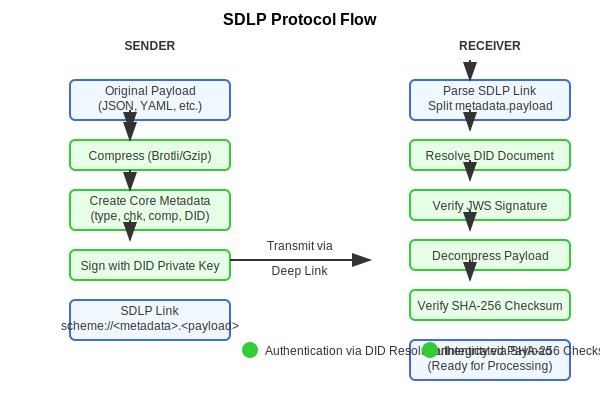
\includegraphics[width=3.5in]{figures/protocol-flow}
% \caption{SDLP Protocol Flow: Sender creates authenticated link, receiver verifies signature and DID before processing payload.}
% \label{fig:protocol-flow}
% \end{figure}

\subsection{Metadata Structure}

The metadata portion contains a JWS Flattened JSON Serialization with the following components:

\textbf{Protected Header:} Contains the cryptographic algorithm (\texttt{alg}) and key identifier (\texttt{kid}). The \texttt{kid} field specifies a complete DID URL pointing to a verification method in the sender's DID document.

\textbf{Payload (Core Metadata):} Contains protocol version (\texttt{v}), sender identifier (\texttt{sid}), payload MIME type (\texttt{type}), compression algorithm (\texttt{comp}), SHA-256 checksum (\texttt{chk}), and optional temporal bounds (\texttt{exp}, \texttt{nbf}).

\textbf{Signature:} Ed25519 signature over the JWS signing input, computed as ASCII(BASE64URL(protected) + '.' + BASE64URL(payload)).

\subsection{Security Model}

SDLP provides the following security guarantees:

\textbf{Authentication:} The DID resolution process and signature verification establish sender identity. Receivers can distinguish between known, trusted DIDs and unknown ones.

\textbf{Integrity:} The SHA-256 checksum in the core metadata, protected by the JWS signature, ensures payload integrity. Any modification to the payload will result in checksum mismatch.

\textbf{Non-repudiation:} Ed25519 signatures provide non-repudiation assuming proper private key protection.

The protocol does not provide:

\textbf{Confidentiality:} Payloads are transmitted in plaintext (though optionally compressed). Applications requiring confidentiality should implement encryption at the payload level.

\textbf{Replay Protection:} While optional temporal bounds (\texttt{exp}, \texttt{nbf}) provide basic replay protection, applications with stronger requirements should implement additional measures.

\section{Implementation}

\subsection{Reference Implementation}

We developed a production-ready TypeScript SDK providing SDLP link creation and verification capabilities. The implementation includes:

\begin{itemize}
    \item Ed25519 cryptographic operations using the \texttt{@noble/ed25519} library
    \item DID resolution supporting \texttt{did:key}, \texttt{did:web}, and extensible architecture for additional methods
    \item Compression support for Brotli, Gzip, and Zstandard algorithms
    \item Comprehensive error handling with standardized error codes
    \item CLI tools for testing and integration
\end{itemize}

The implementation prioritizes security through input validation, safe parsing, and protection against common vulnerabilities like JSON injection and malformed data attacks.

\subsection{Payload Capacity Analysis}

SDLP achieves significant efficiency improvements over naive JWT-in-URL approaches through architectural optimization:

\textbf{Traditional JWT Approach:} Payload → Base64URL → JWT → Base64URL results in $\approx 1.78\times$ size multiplication (78\% overhead).

\textbf{SDLP Approach:} Payload → Compression → Base64URL results in $\approx 1.33\times$ size multiplication (33\% overhead).

For a 32KB URL limit with estimated 1KB metadata overhead, SDLP provides approximately 23KB of compressed payload capacity, achieving 72\% payload efficiency.

\section{Performance Evaluation}

\subsection{Experimental Setup}

We evaluated SDLP performance using a comprehensive benchmark suite on macOS ARM64 with Node.js v23.7.0. Tests measured link creation, verification, and capacity utilization across different payload sizes (32B, 256B, 1KB) with and without compression.

\subsection{Link Creation Performance}

Link creation performance remains consistent across payload sizes:

\begin{table}[!t]
\caption{Link Creation Performance}
\label{tab:creation-performance}
\centering
\begin{tabular}{@{}lcc@{}}
\toprule
Payload Size & Average Time (ms) & Throughput (ops/sec) \\
\midrule
32B (uncompressed) & 0.09 & 11,600 \\
256B (uncompressed) & 0.11 & 9,200 \\
1KB (uncompressed) & 0.10 & 9,800 \\
256B (Brotli) & 0.11 & 9,000 \\
1KB (Brotli) & 0.11 & 9,100 \\
\bottomrule
\end{tabular}
\end{table}

The consistent sub-millisecond creation times demonstrate that cryptographic operations dominate performance rather than payload processing, making SDLP suitable for real-time applications.

\subsection{Verification Performance}

Link verification shows slightly higher latency due to DID resolution and signature validation:

\begin{table}[!t]
\caption{Link Verification Performance}
\label{tab:verification-performance}
\centering
\begin{tabular}{@{}lcc@{}}
\toprule
Payload Size & Average Time (ms) & Throughput (ops/sec) \\
\midrule
32B & 0.32 & 3,100 \\
256B & 0.35 & 2,900 \\
1KB & 0.38 & 2,600 \\
\bottomrule
\end{tabular}
\end{table}

These results include DID document parsing and Ed25519 signature verification. In production scenarios, DID document caching could further improve performance.

\subsection{Compression Effectiveness}

Brotli compression provides significant space savings for larger payloads:

\begin{table}[!t]
\caption{Compression Analysis}
\label{tab:compression}
\centering
\begin{tabular}{@{}lccc@{}}
\toprule
Payload & Uncompressed & Compressed & Reduction \\
\midrule
32B & 789B total & N/A & 0\% \\
256B & 1,117B total & 1,009B total & 9.7\% \\
1KB & 2,233B total & 1,433B total & 35.9\% \\
\bottomrule
\end{tabular}
\end{table}

Compression effectiveness increases with payload size, with 1KB payloads achieving 35.9% URL length reduction.

\section{Security Analysis}

\subsection{Threat Model}

SDLP addresses threats from attackers who can:
\begin{itemize}
    \item Intercept and modify deep links in transmission
    \item Generate malicious deep links impersonating legitimate senders
    \item Attempt replay attacks using previously valid links
\end{itemize}

SDLP does not address threats from:
\begin{itemize}
    \item Compromised sender private keys
    \item Malicious payload content (applications must implement content validation)
    \item Side-channel attacks on cryptographic implementations
\end{itemize}

\subsection{Cryptographic Security}

SDLP leverages established cryptographic primitives:

\textbf{Ed25519:} Provides 128-bit security level with resistance to timing attacks and deterministic signatures~\cite{ed25519}.

\textbf{SHA-256:} Ensures collision resistance for payload integrity verification~\cite{sha256-security}.

\textbf{JWS:} Follows RFC 7515 for signature format and verification procedures.

\subsection{DID Security Considerations}

Different DID methods provide varying security properties:

\textbf{did:key:} Self-contained keys provide immediate verification but lack revocation mechanisms.

\textbf{did:web:} Web-based keys enable updates and revocation but depend on DNS and HTTPS security.

Applications should choose DID methods appropriate to their security requirements and threat models.

\section{Applications and Use Cases}

SDLP addresses security requirements across various application domains:

\textbf{AI Prompt Sharing:} Authenticated prompts prevent injection attacks and ensure prompt provenance in AI applications.

\textbf{Configuration Distribution:} Development tools can securely distribute configuration data with verified authenticity.

\textbf{Cross-Application Authentication:} Applications can exchange authentication tokens through verified deep links.

\textbf{IoT Device Control:} Authenticated commands prevent unauthorized device manipulation.

\textbf{Data Sharing:} Peer-to-peer applications can exchange small data objects with integrity guarantees.

\section{Limitations and Future Work}

Current limitations include:

\textbf{Key Management:} Applications must implement secure private key storage and protection mechanisms.

\textbf{DID Resolution Dependencies:} Network-based DID methods require connectivity and may introduce latency.

\textbf{URL Length Constraints:} While optimized, SDLP still faces fundamental URL length limitations across different platforms.

Future work directions include:

\textbf{Standardization:} Pursuing formal standardization through appropriate standards bodies.

\textbf{Additional DID Methods:} SDK support for emerging DID methods like \texttt{did:peer} for peer-to-peer scenarios (protocol already supports any W3C DID method).

\textbf{Advanced Features:} Investigating selective disclosure, zero-knowledge proofs, and enhanced privacy features.

\textbf{Performance Optimization:} Exploring cryptographic algorithm alternatives and implementation optimizations.

\section{Conclusion}

The Secure Deep Link Protocol addresses critical security gaps in deep link communication through a lightweight, efficient design that provides authentication and integrity verification without centralized dependencies. Our performance evaluation demonstrates that SDLP achieves sub-millisecond operation latencies while maintaining 72\% payload efficiency within URL constraints.

SDLP's integration with Decentralized Identifiers enables trustless authentication scenarios while maintaining compatibility with existing mobile platforms and URL schemes. The protocol's flexibility in supporting various payload types and compression algorithms makes it suitable for diverse applications from AI prompt sharing to IoT device control.

The open-source reference implementation and comprehensive benchmarking suite facilitate adoption and further research. As deep links become increasingly prevalent for inter-application communication, SDLP provides a foundation for secure, authenticated data transmission that scales from simple configuration sharing to complex multi-party scenarios.

\section*{Acknowledgments}

The author thanks the W3C DID Working Group for their work on Decentralized Identifier specifications, and the broader cryptographic community for developing the foundational primitives that enable secure protocols like SDLP.

\bibliographystyle{IEEEtran}
\bibliography{references}

\end{document}
